
% FIGURES -------------------------------------------------------
% Figures
% ranked improvement - FULL
\begin{figure}[H]
    \centering
    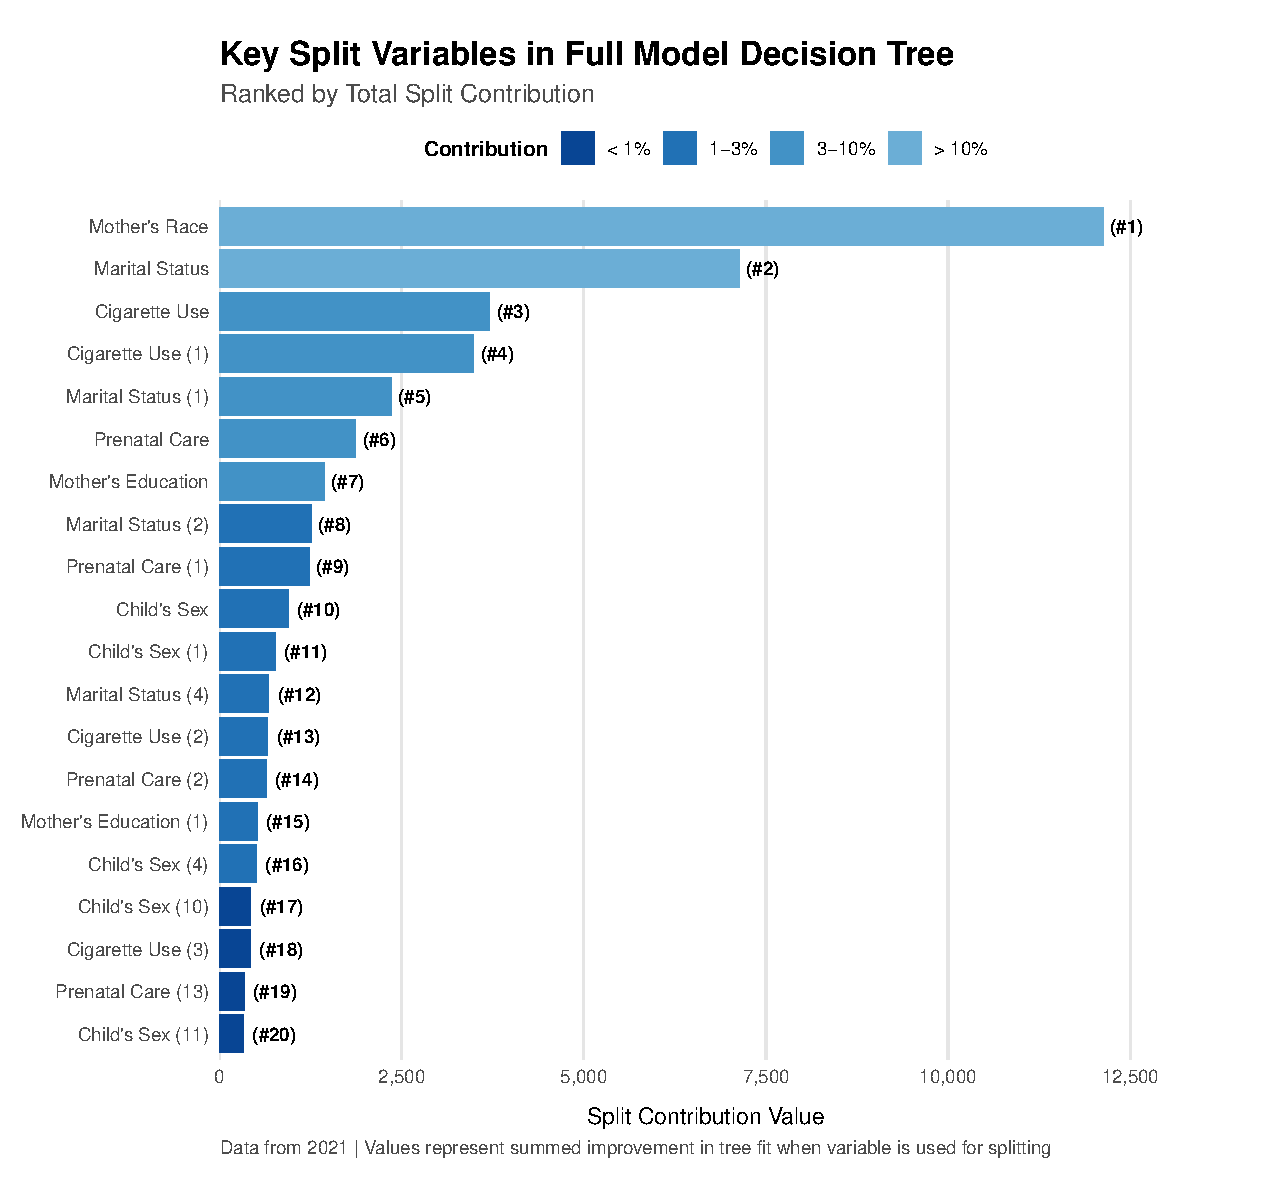
\includegraphics[width=1\linewidth]{chapters/chapter3/figures/improvement/tree_split_contribution_top20_Full Model.pdf}
    \caption{Full Model Ranked Improvement. Rankings represent summed reduction in deviance (improvement in model fit) across all nodes where each variable is used for splitting in the tree. Plot only displays top 20 ranked variables.}
    \label{fig:full-model-ranked-imp}
\end{figure}

% ranked improvement - LBW
\begin{figure}[H]
    \centering
    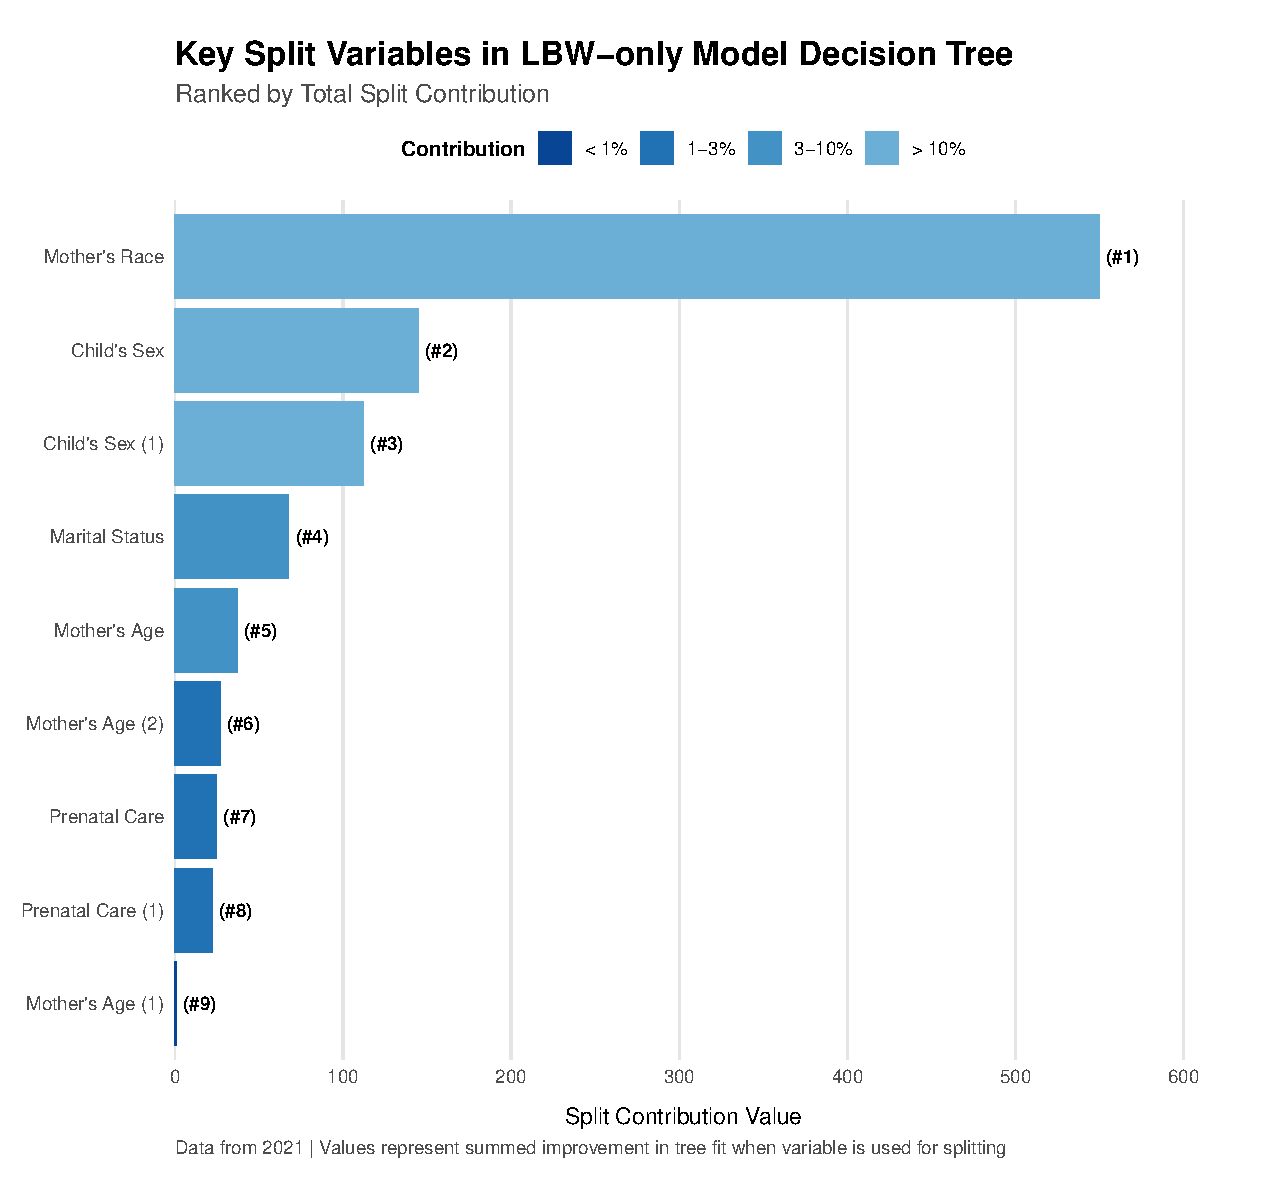
\includegraphics[width=1\linewidth]{chapters/chapter3/figures/improvement/tree_split_contribution_top9_LBW-only Model.pdf}
    \caption{LBW-only Model Ranked Improvement. Rankings represent summed reduction in deviance (improvement in model fit) across all nodes where each variable is used for splitting in the tree. Plot displays all ranked variables.}
    \label{fig:lbw-model-ranked-imp}
\end{figure}

% % First barplot figure
% \begin{figure}[H]
%     \centering
%     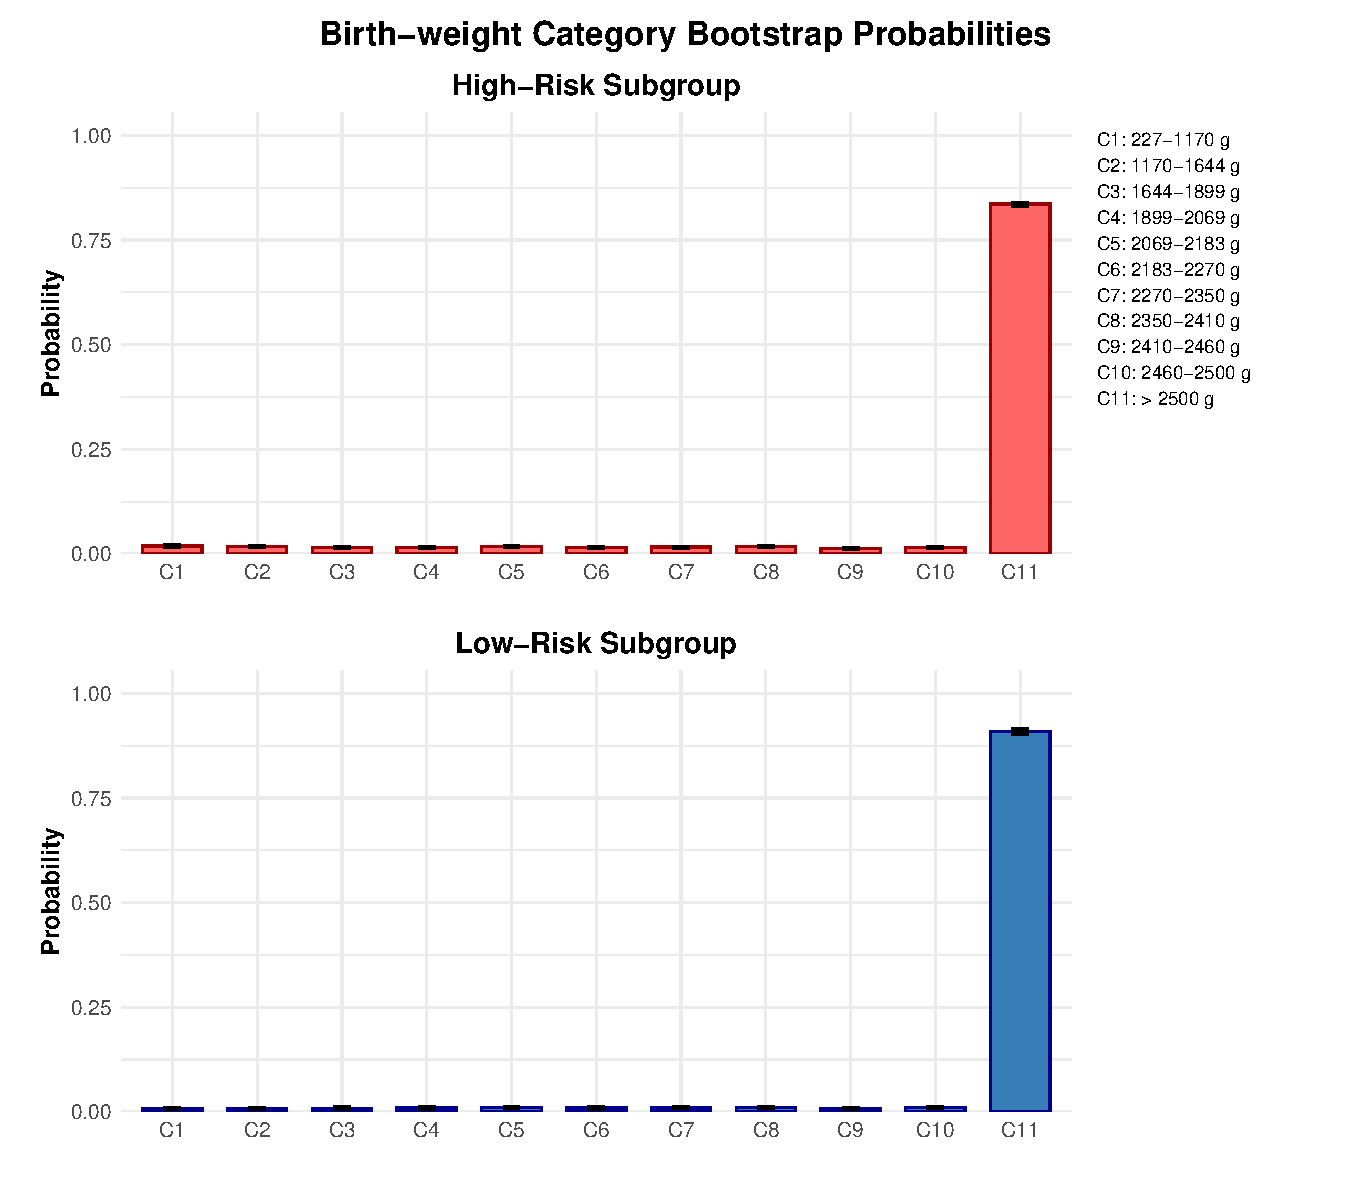
\includegraphics[width=1\textwidth]{chapters/chapter3/figures/high_low_risk_full.pdf}
%     \caption{Full model: Aggregated mean probability estimates by birth-weight category across $B$ bootstraps, showing the distribution of predicted probabilities for high and low risk subgroups with 95\% percentile intervals.}
%     \label{fig:high-low-risk-full}
% \end{figure}

% % First barplot figure (without NBW)
% \begin{figure}[H]
%     \centering
%     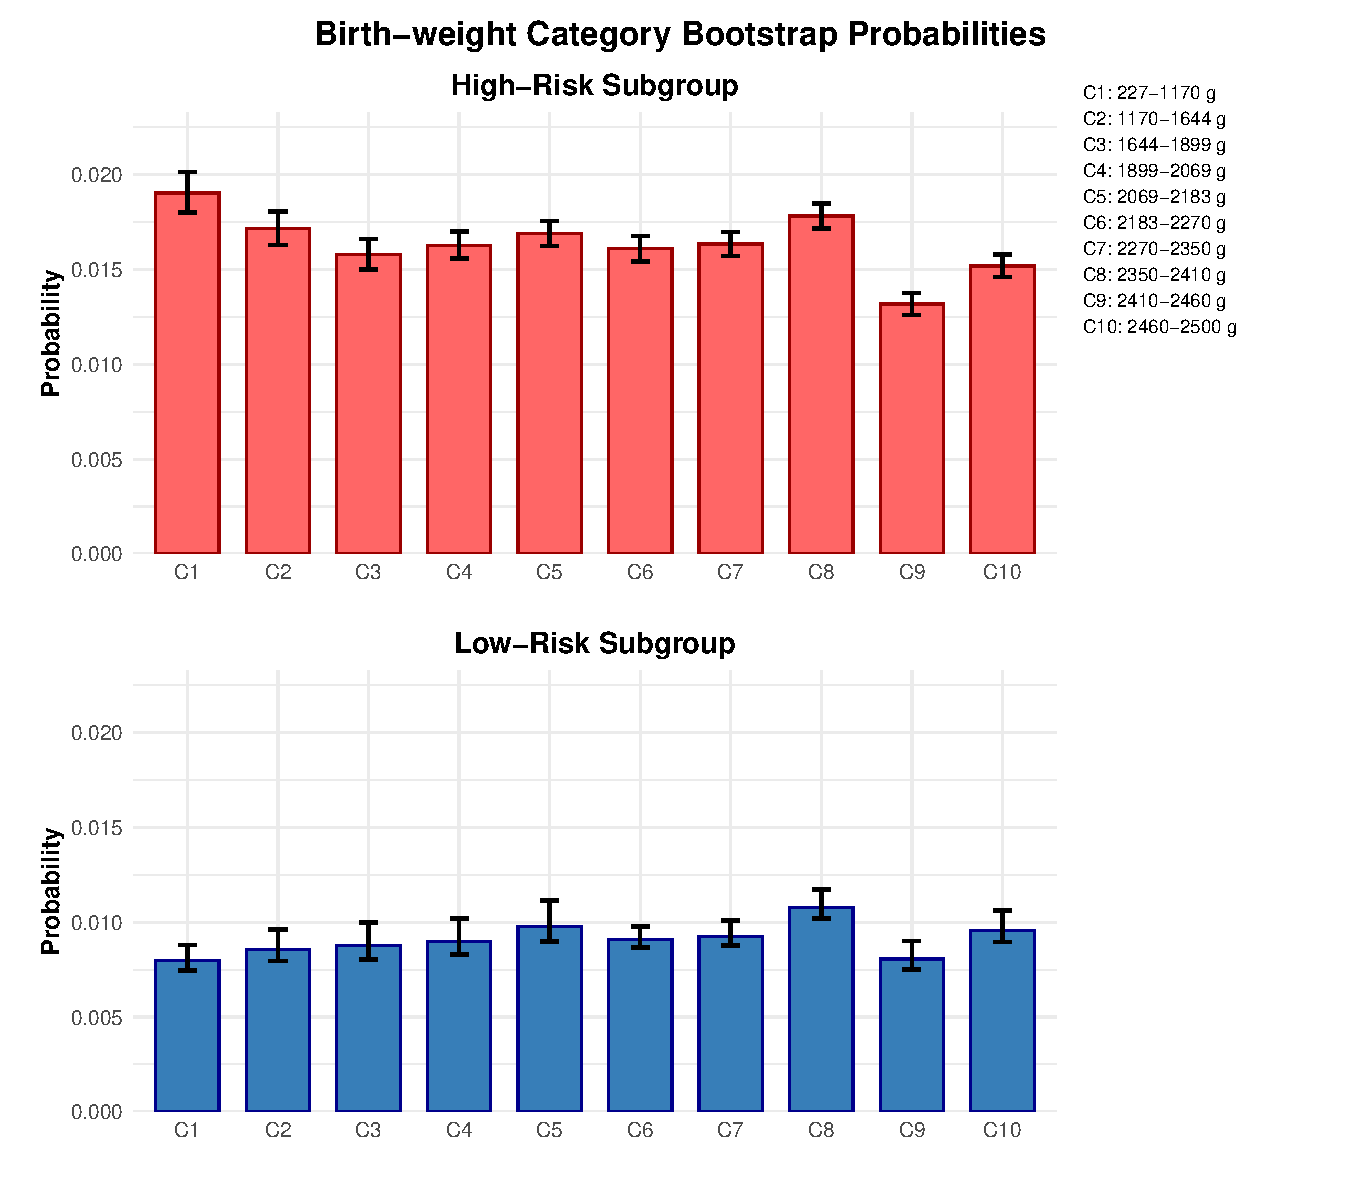
\includegraphics[width=1\textwidth]{chapters/chapter3/figures/high_low_risk_full_without_NBW.pdf}
%     \caption{Full model (without NBW birth-weight column): Aggregated mean probability estimates by birth-weight category across $B$ bootstraps, showing the distribution of predicted probabilities for high and low risk subgroups with 95\% percentile intervals.}
%     \label{fig:high-low-risk-full-w/o-NBW}
% \end{figure}

% % Second barplot figure
% \begin{figure}[H]
%     \centering
%     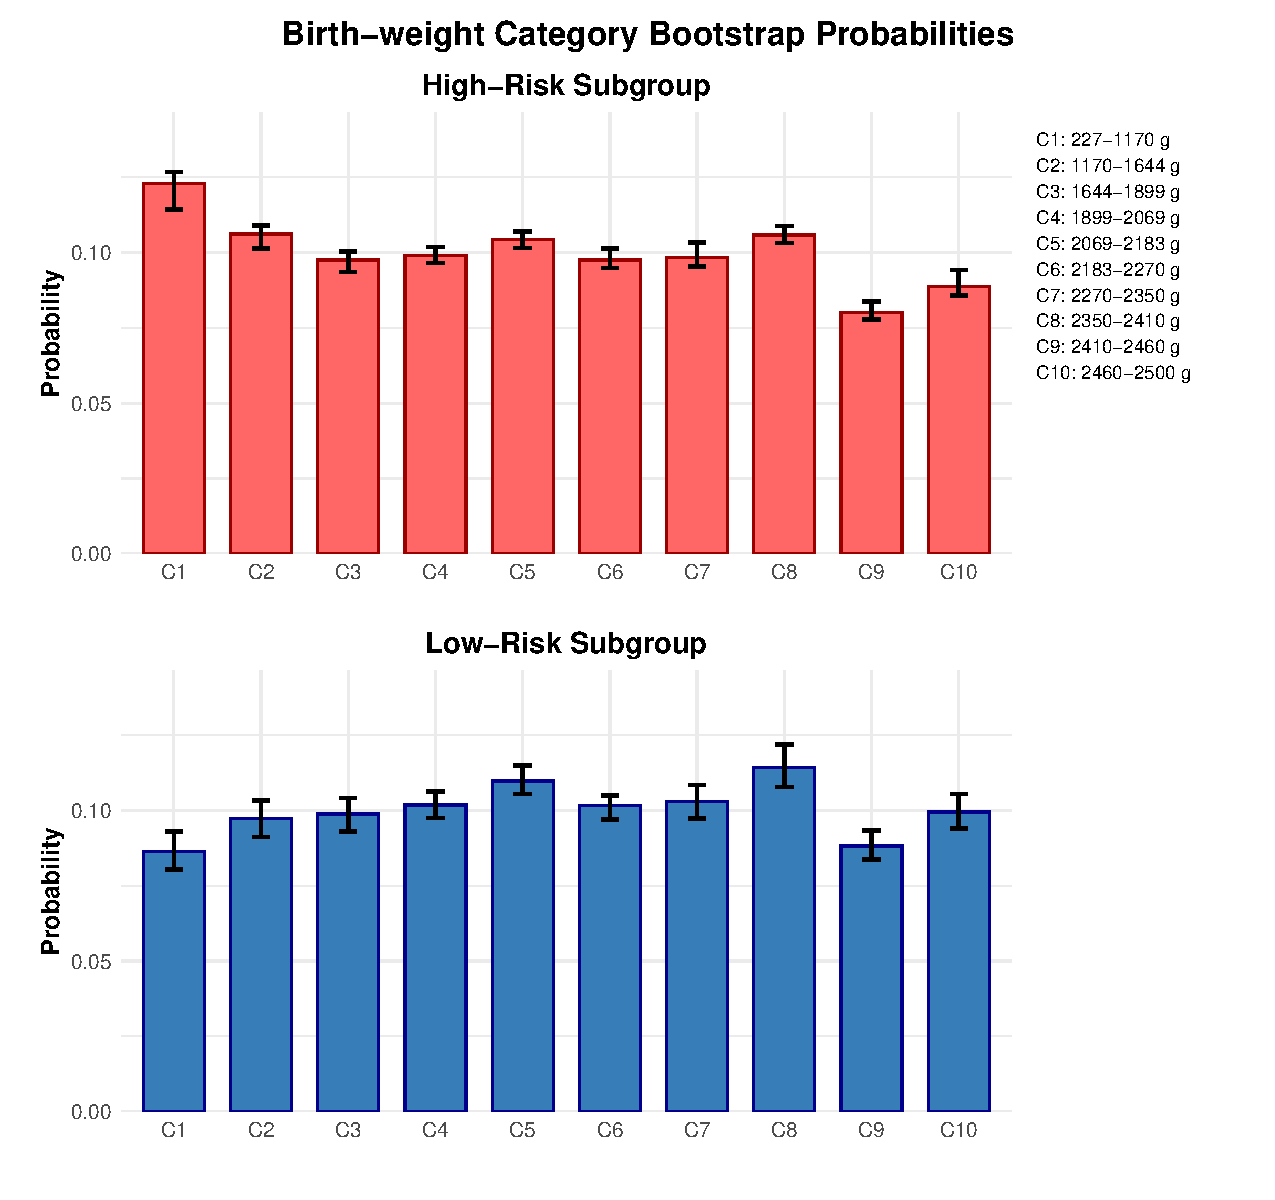
\includegraphics[width=1\textwidth]{chapters/chapter3/figures/high_low_risk_small.pdf}
%     \caption{LBW-only model: Aggregated mean probability estimates by birth weight category across $B$ bootstraps, showing the distribution of predicted probabilities for high and low risk subgroups with 95\% percentile intervals.}
%     \label{fig:high-low-risk-lbw}
% \end{figure}

% ─────────────────────────────────────────────────────────────────────────
% Full + NBW (11 categories)
\begin{figure}[H]
  \centering
  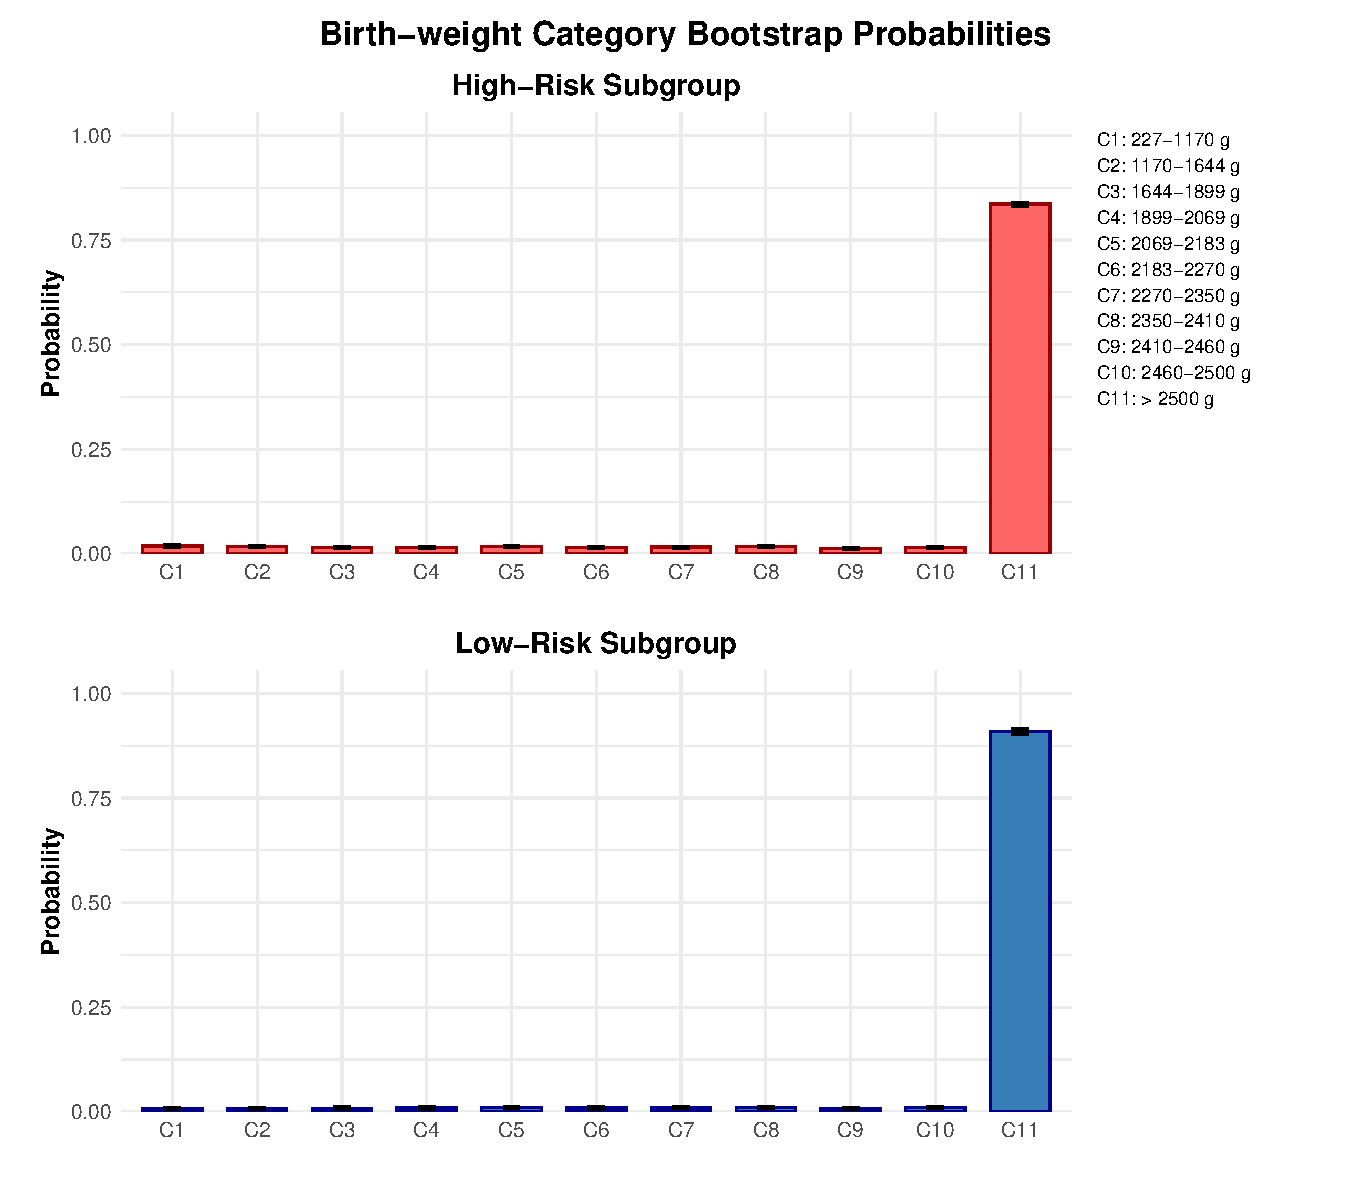
\includegraphics[width=\textwidth]{chapters/chapter3/figures/high_low_risk_full.pdf}
  \caption{Full model: Mean bootstrap probability for each birth-weight category (C1–C11) in the high- and low-risk subgroups. Error bars show the 95 \% percentile interval over the $B$ bootstrap trees.}
  \label{fig:high-low-risk-full}
\end{figure}

% ─────────────────────────────────────────────────────────────────────────
% Full - NBW (C11 removed, 10 categories)
\begin{figure}[H]
  \centering
  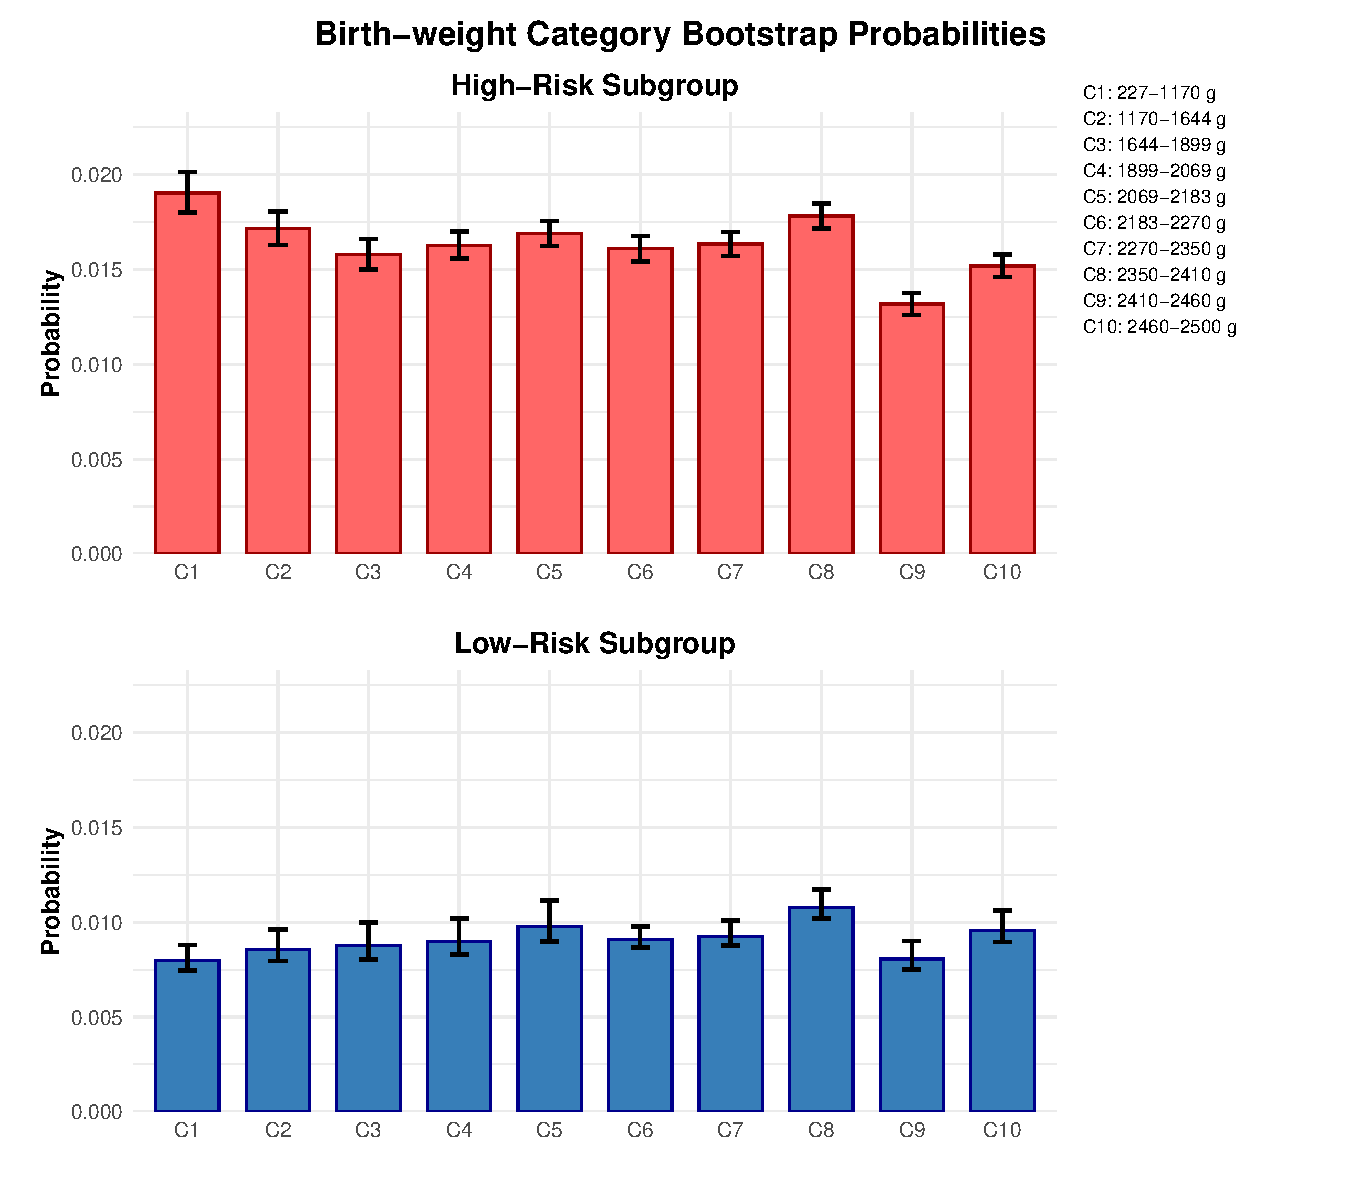
\includegraphics[width=\textwidth]{chapters/chapter3/figures/high_low_risk_full_without_NBW.pdf}
  \caption{Full model (excluding the NBW column): Probability estimates and intervals are as in Fig.~\ref{fig:high-low-risk-full}.}
  \label{fig:high-low-risk-full-w/o-NBW}
\end{figure}

% ─────────────────────────────────────────────────────────────────────────
% LBW-only (10 categories)
\begin{figure}[H]
  \centering
  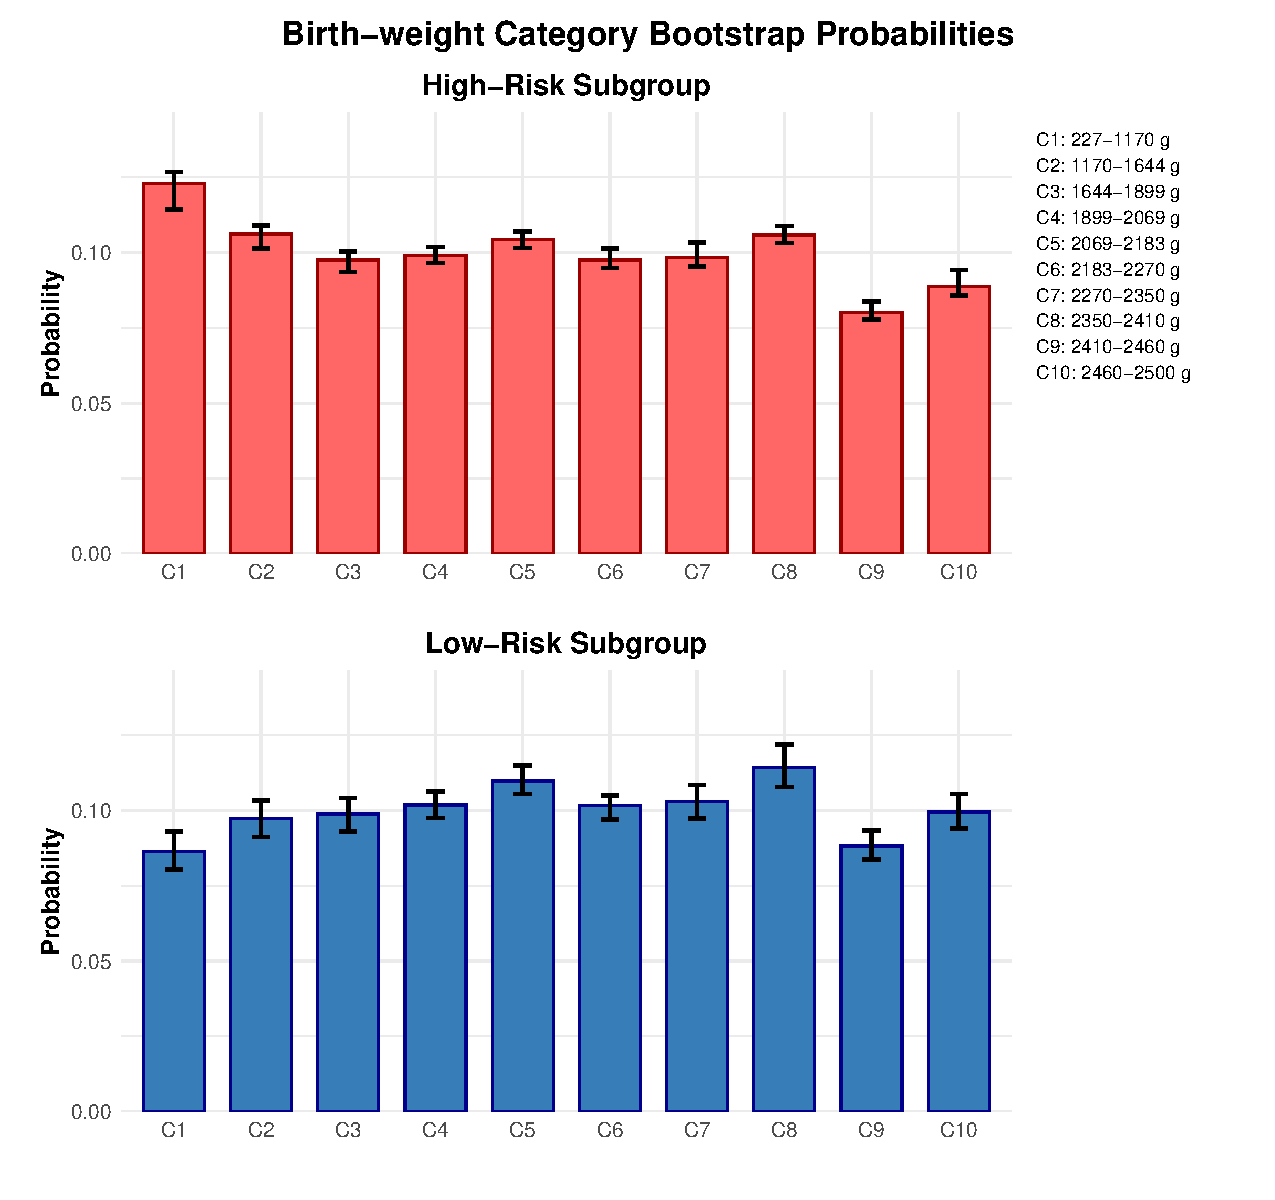
\includegraphics[width=\textwidth]{chapters/chapter3/figures/high_low_risk_small.pdf}
  \caption{LBW-only model (10 categories):  Mean bootstrap probability for each birth-weight category in the two risk groups with 95\% percentile intervals.}
  \label{fig:high-low-risk-lbw}
\end{figure}

% Depth distributions — Full model
\begin{figure}[H]
    \centering
    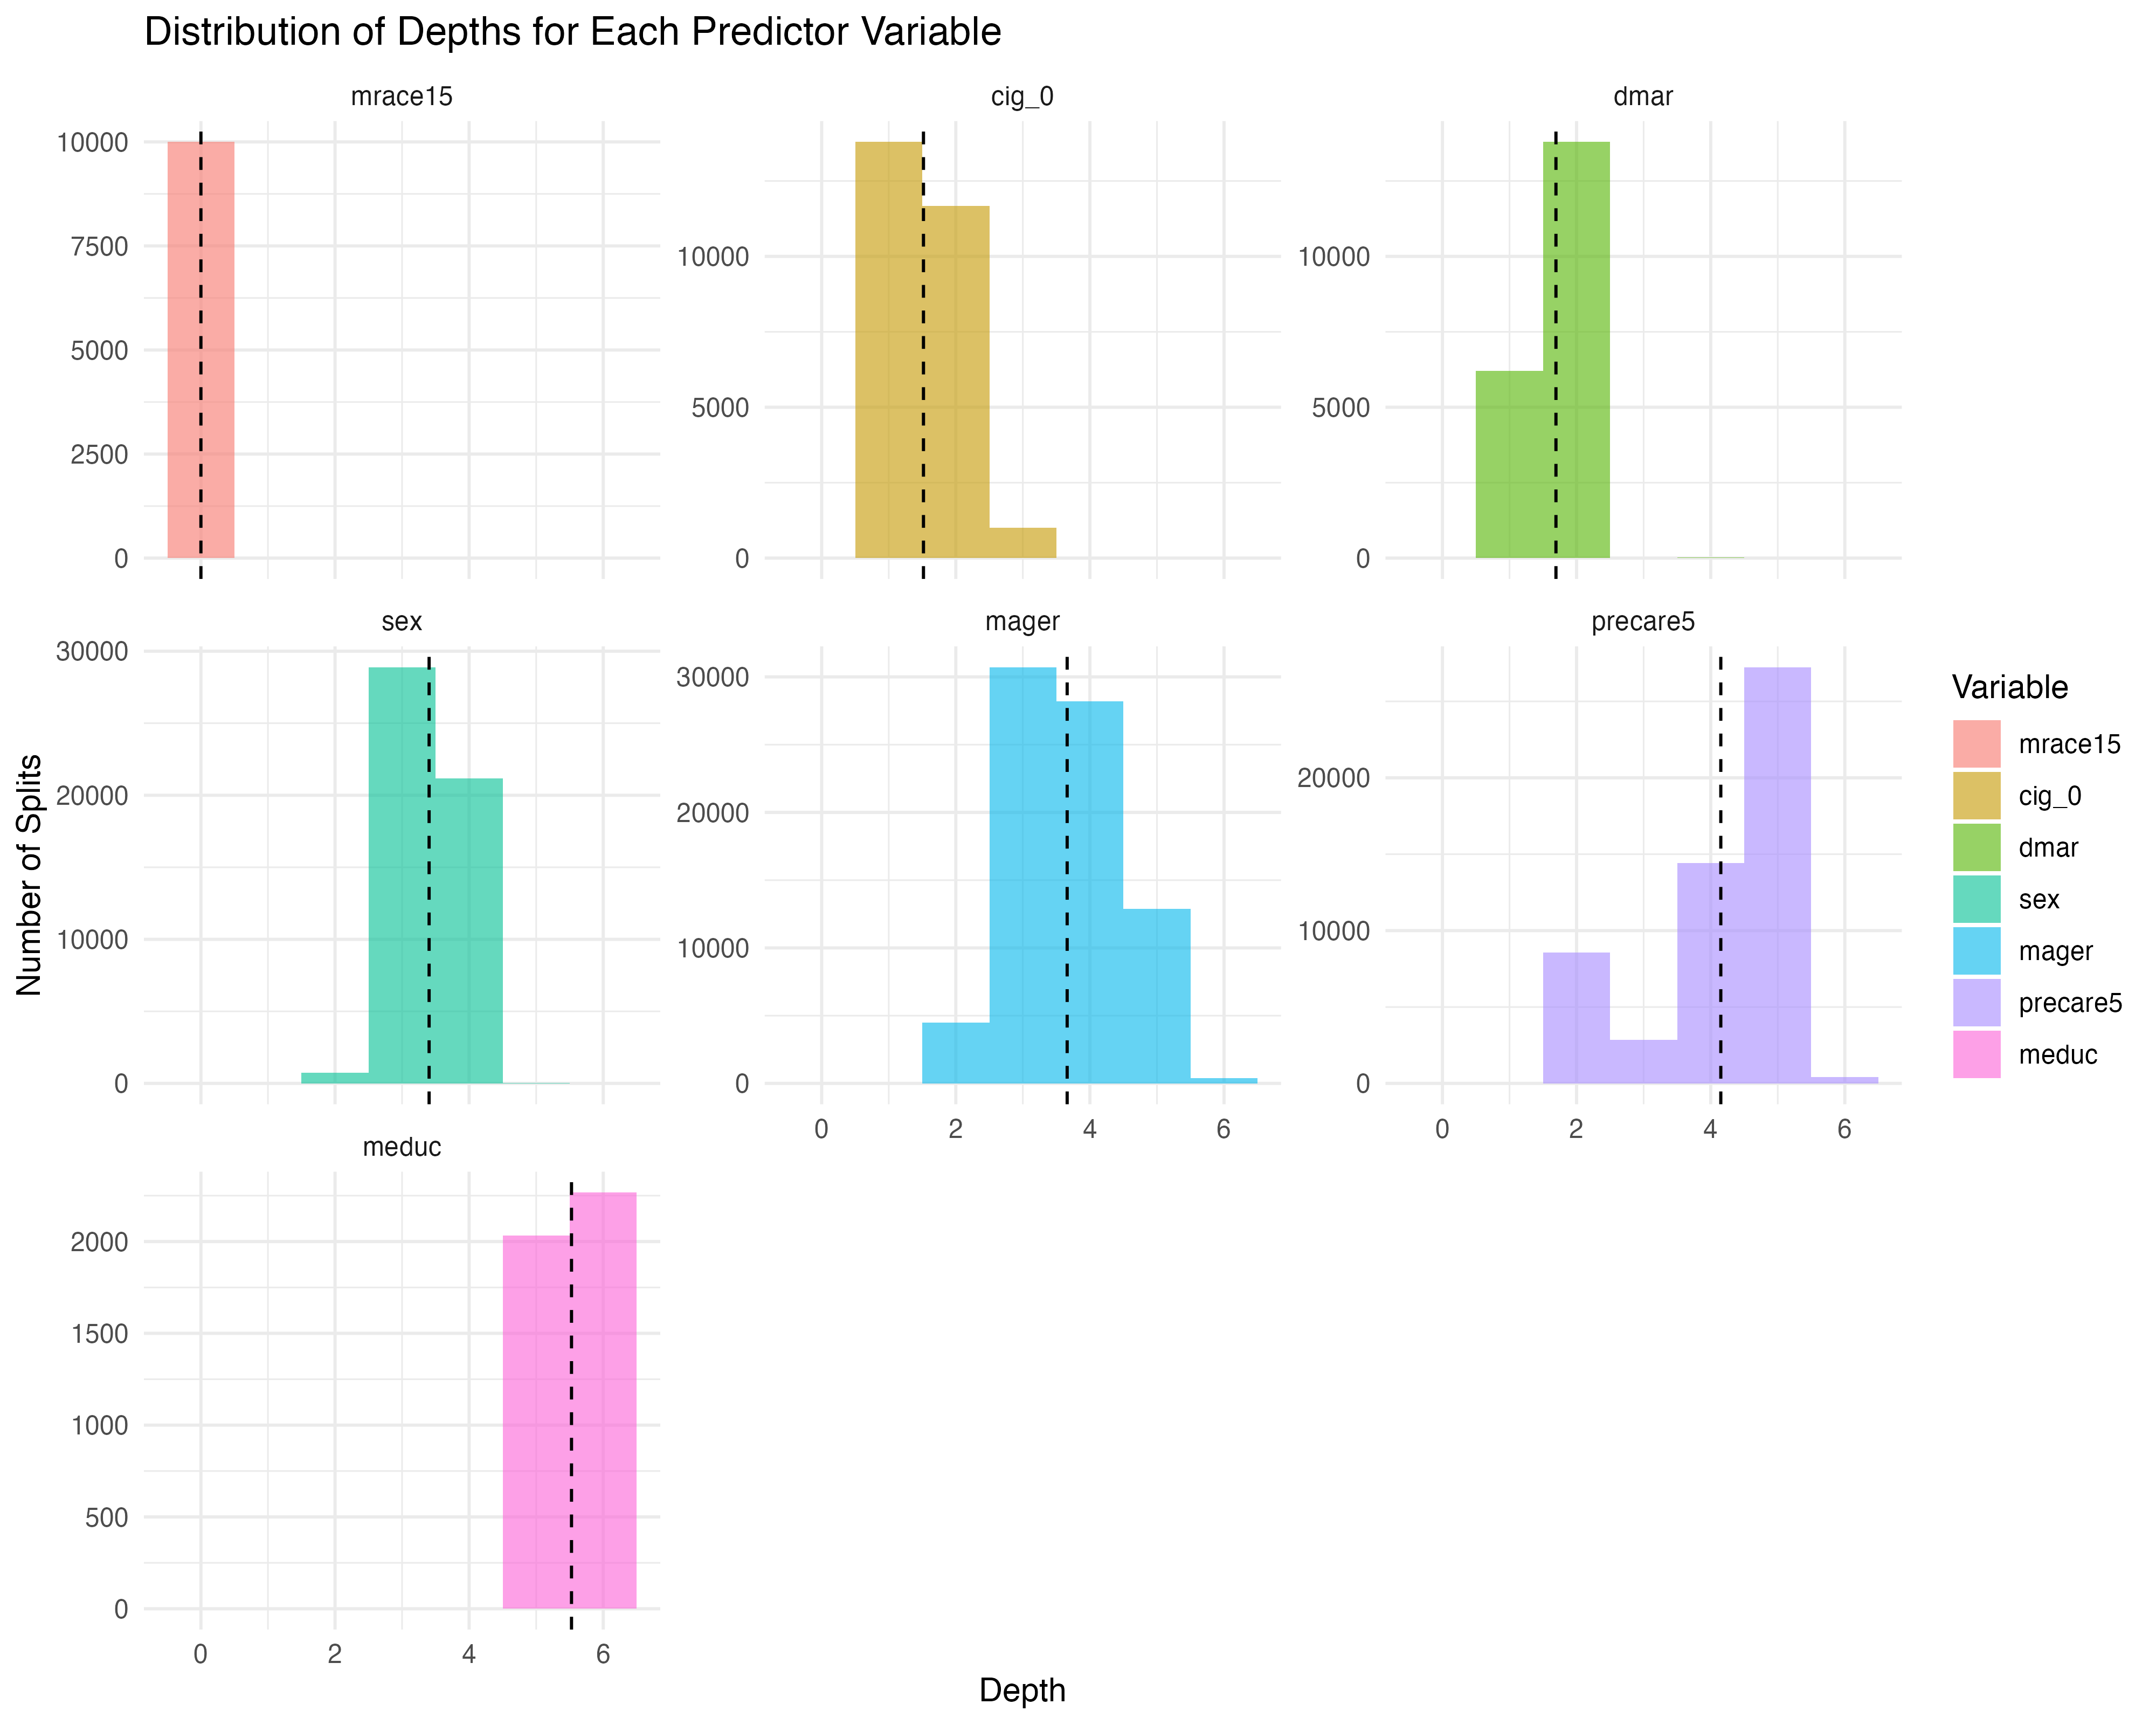
\includegraphics[width=1.0\textwidth]{chapters/chapter3/figures/boot/depth_distributions.png}
    \caption{Full model: Distribution of variable depths across the ensemble. Each panel shows a histogram indicating how frequently a given variable appears at each tree depth, where depth 0 corresponds to the root node. Variables closer to the root are generally more important in the model.}
    \label{fig:var-depth-distributions-full}
\end{figure}

% Depth distributions — LBW-only model
\begin{figure}[H]
    \centering
    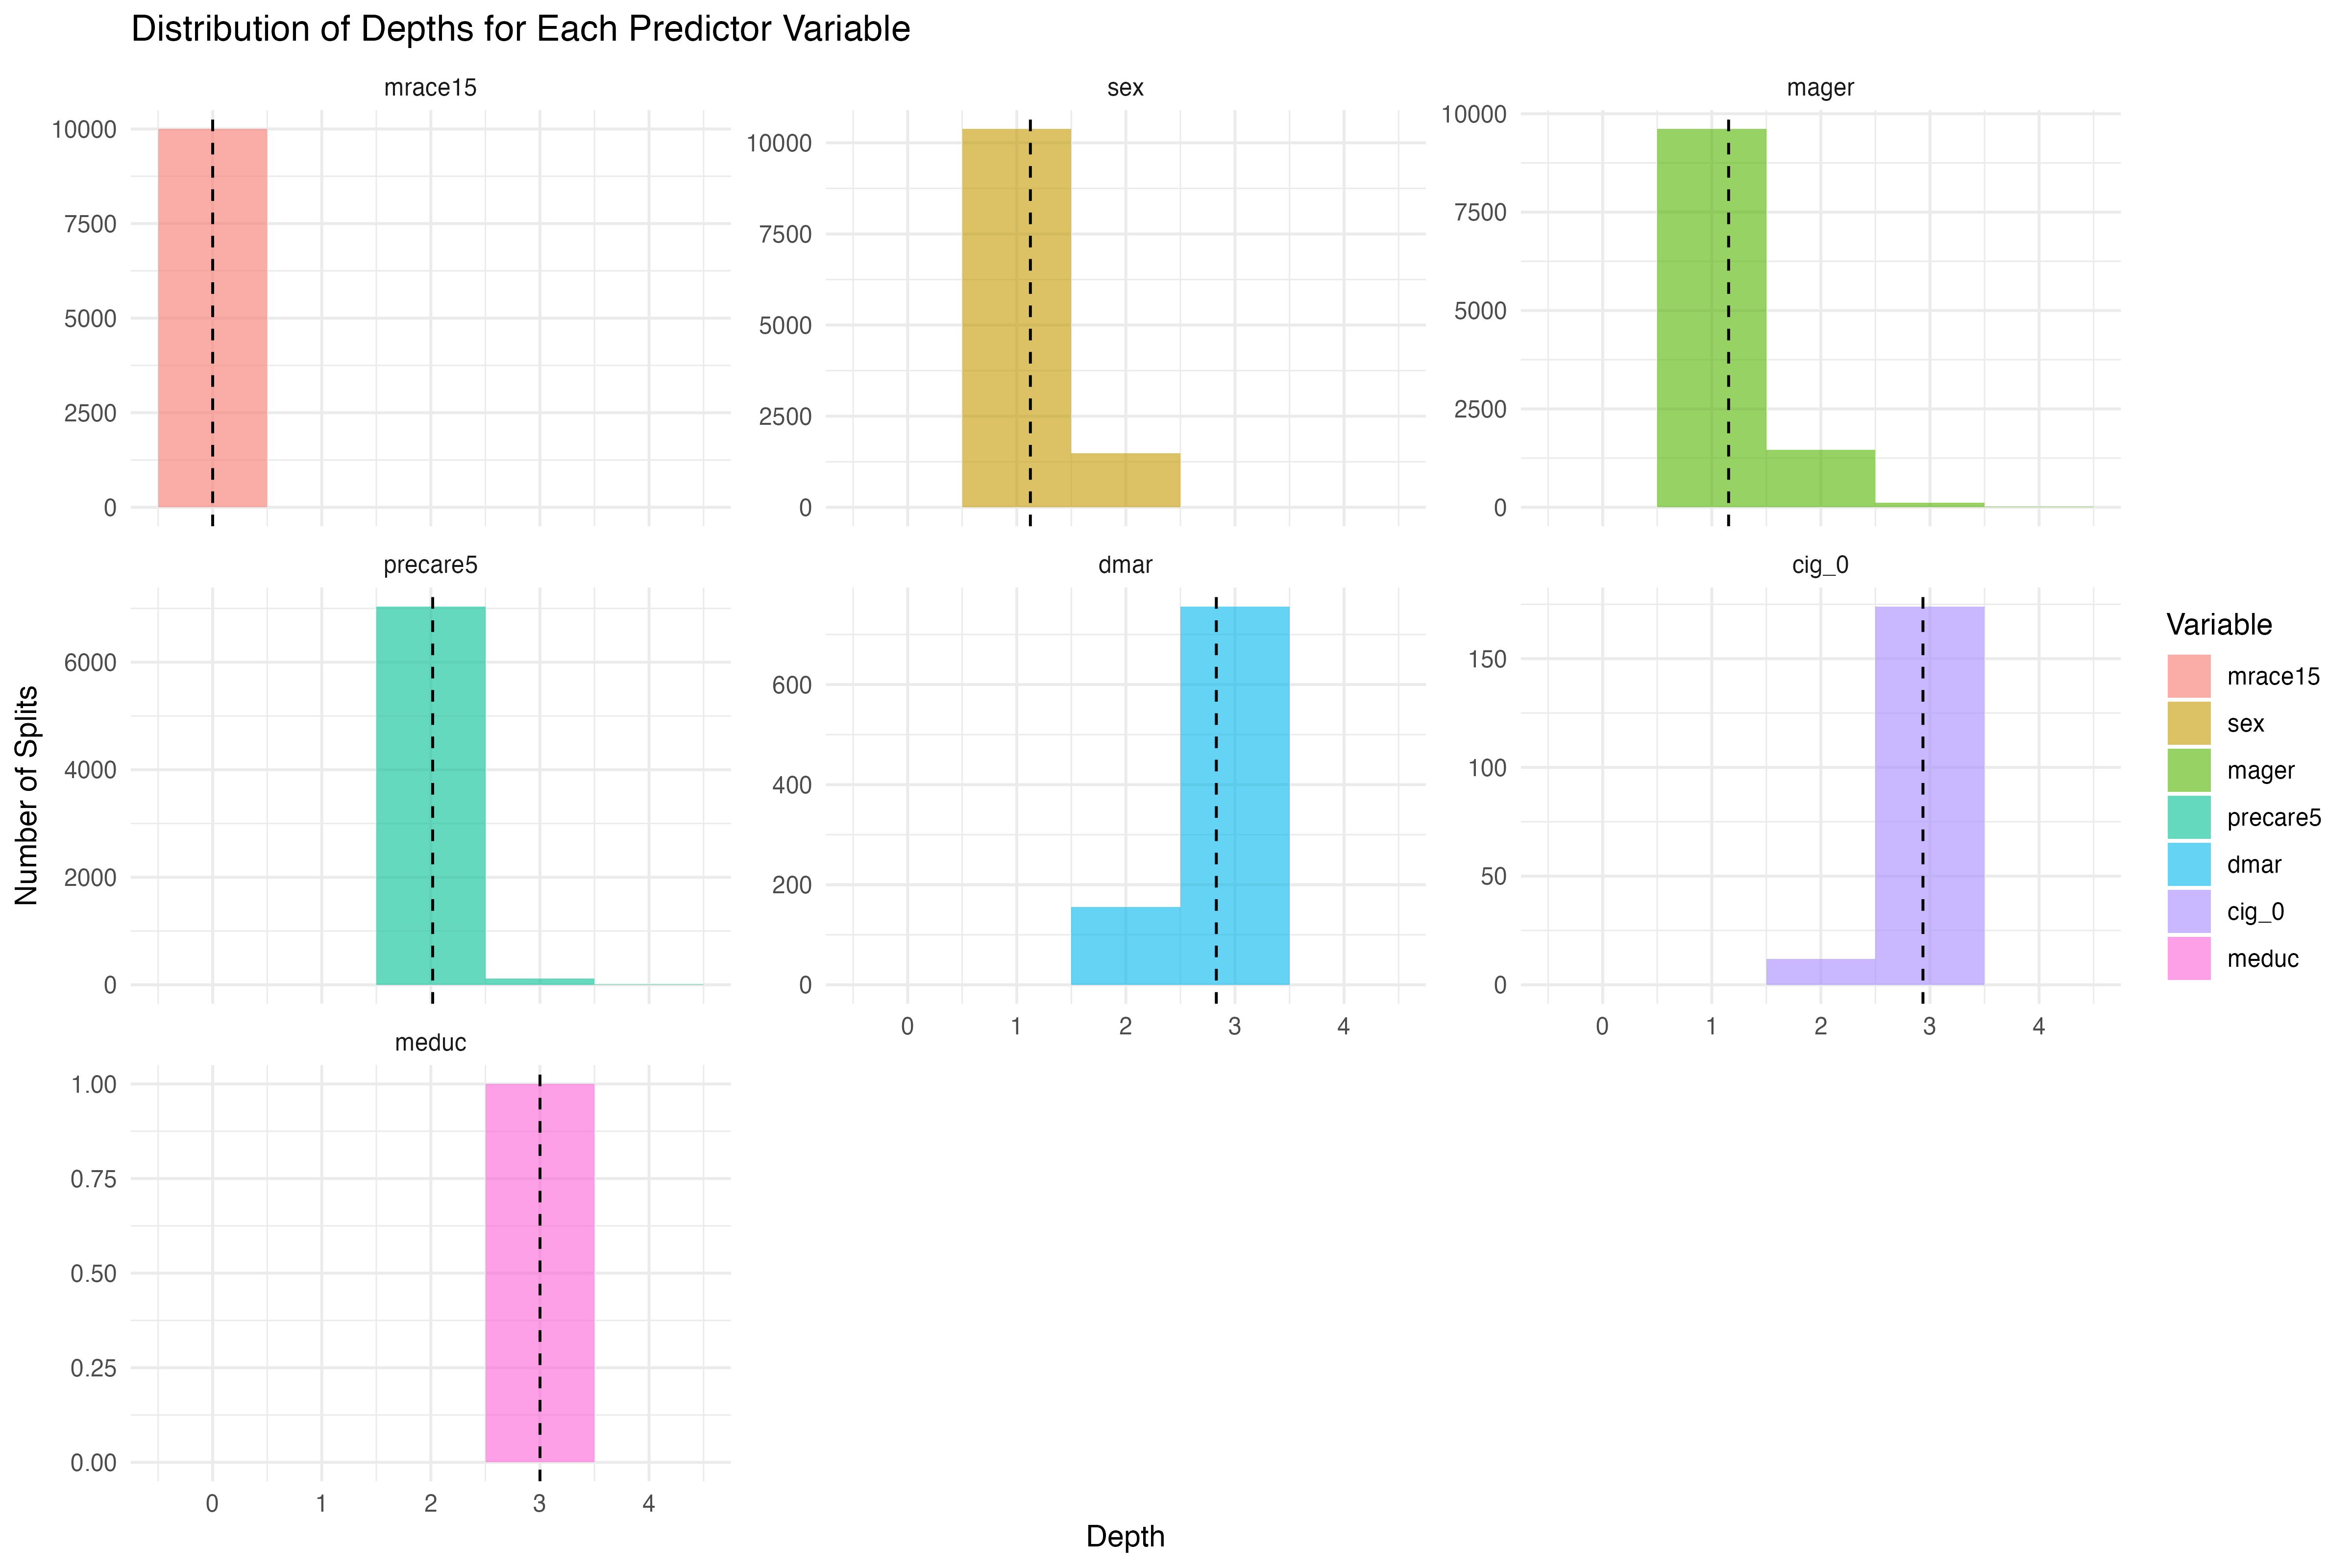
\includegraphics[width=1.0\textwidth]{chapters/chapter3/figures/boot/depth_distributions_2.png}
        \caption{LBW-only model: Distribution of variable depths across the ensemble. Each panel shows a histogram indicating how frequently a given variable appears at each tree depth, where depth 0 corresponds to the root node. Variables closer to the root are generally more important in the model.}
    \label{fig:var-depth-distributions-lbw}
\end{figure}
